\chapter{Sizing of Hardware}
\label{chap:sizing}
We looked at two designs in Chapter \ref{chap:mech_design}. This chapter describes some simulations done
for the sizing of various components. The major parts of this process are,
\begin{enumerate}
\item
Masses of the platform and the leg
\item
Dimensions of the reaction wheel based on the above masses
\item
Choice of winding and reaction wheel motors
\end{enumerate}

\section{$2$ mass problem}
\begin{figure}[!h]
\centering
\begin{tikzpicture}[scale=0.45]
\draw (-3,0) -- (3,0);
\foreach \x in {-2.5,-2,...,2.5}
\draw (\x,0) -- (\x+0.5,-0.5);

\path (-2,7) coordinate(M1);
\path (2,10) coordinate(M2);
\path (-0.6,2) coordinate(m1);
\path (0.6,3.2) coordinate(m2);

\draw [thick](M1) rectangle (M2) node[midway]{\huge{$M$}};
\draw [thick](m1) rectangle (m2) node[midway]{\Large{$m$}};

\path (-2.5,0) coordinate (O);
\path (-2.5,2.6) coordinate (SPL);
\path (-2.5,8.5) coordinate (H);

\draw[<->] [semithick](O)++(-0.5,0) -- (-3,8.5) node[midway, left]{$H$};
\draw[<->] [semithick](SPL) -- (H) node[midway, right]{$l_0$};


\draw[snake=coil, segment amplitude=8pt] (0,3.2) -- (0,7) node[midway,right=2ex]{$k$};
\end{tikzpicture}
\caption[2 mass problem]{2 mass problem \cite{simit}}
\label{fig:4_2mass}
\end{figure}
The basic idea behind a hopper is like that of the 2 masses connected by a spring problem. If the system shown in Fig.
\ref{fig:4_2mass} is allowed to fall from a height, the heavier mass pulls the smaller mass with it back into the air
after impact. Every cycle is accompanied by a loss in energy due to the inelastic impact of the smaller mass with the
ground. If we pump this energy back into the system using an external agent in every cycle, we can ensure sustained
hopping at the chosen height. The 2 mass problem can thus be taken as a basis to compute the range of values of masses
for acceptable performance. The following assumptions have been used in the simulation that follows,
\begin{enumerate}
\item
Dropping height (H) : 0.6 m
\item
Spring constant (k) : 300 N/m
\item
Spring relaxed length ($l_0$) : 0.3 m
\item
Trapezoidal profile for $\omega$ of the winding motor (constant $\alpha$ at the start and end)
\item
Design 1 was used as the base for this simulation. It is expected that the total torque requirements will
reduce due to the mechanical advantage provided by the rack and pinion design as shown in Fig. \ref{fig:3_seth_design}.
\item
Neglect energy loss due to friction
\end{enumerate}
It is seen from Fig. \ref{fig:4_2mass} that if $h_i$ are progressive heights, we have the relation,
\begin{equation}
h_n = \frac{Mh_{n-1} + ml_0}{M + m}
\end{equation}
\begin{equation}
\label{eqn:4_eloss}
E_{loss} = \frac{Mg\;(H-l_0)}{1 + M/m}
\end{equation}

\begin{figure}[!h]
\centering
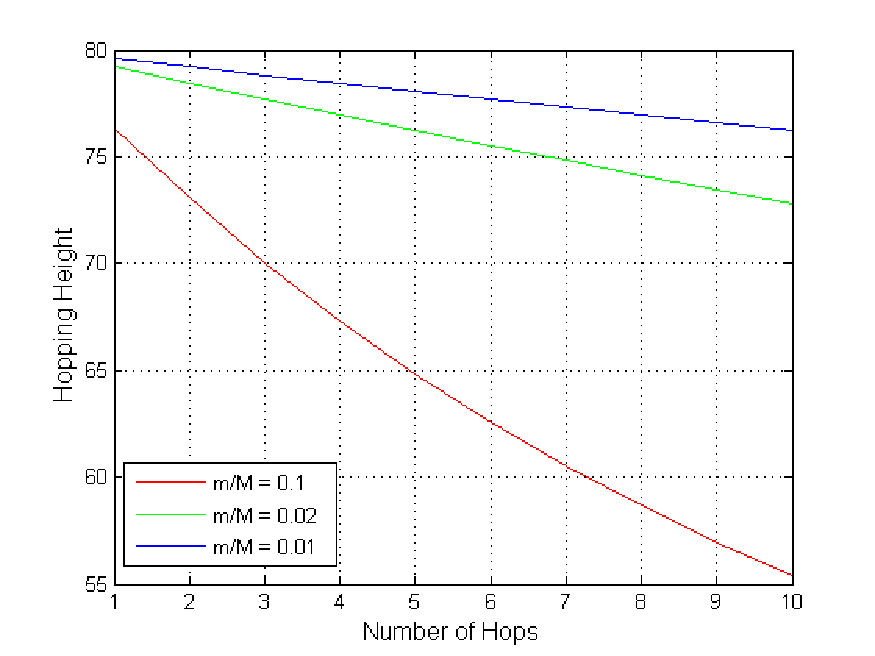
\includegraphics[scale=0.8]{fig/2mass_hopheight.pdf}
\caption{Hopping height for different M/m}
\label{fig:4_hopping_height}
\end{figure}
From Fig. \ref{fig:4_hopping_height}, it is seen that larger the ratio M/m, i.e. smaller the leg
mass, less is the loss in energy resulting in more number of hops. This is also seen for a increasing M. We would however,
like the M to be within limit too as we will also need to pump in extra energy into the system if the desired hopping
height is more than the starting height.\\
\begin{figure}[!h]
\centering
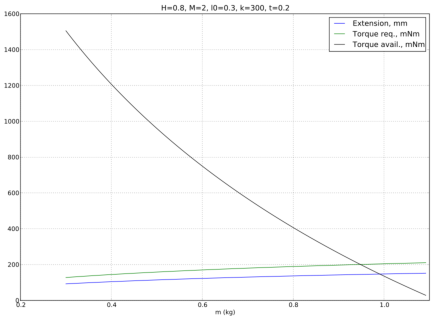
\includegraphics[scale=1.5]{fig/2mass_m.pdf}
\caption{Torque variation with m}
\label{fig:4_torque2mass}
\end{figure}

Fig. \ref{fig:4_torque2mass} shows the required torque  for extending springs to compensate the energy lost during impact fully within 0.2 sec. This simulation has been plotted for Design 1 from Chapter \ref {chap:mech_design} with a pulley radius of 2 cms. It is
observed that m is the single most important parameter in hopper design. The required torque is a very strong function of the leg mass. As this mass increases, we need a larger motor to satisfy torque requirements. It is noted that a value of about 0.4--0.6 kg
can be called a reasonable estimate for the leg mass as we can easily choose a motor delivering the required torque for these values.\\

It is also seen that an extension of about 11 cms with a single spring of k = 300 Nm is needed to compensate the energy loss for 
hopping heights of 80 cms. So we should ensure that we can provide a maximum extension around 15 cms.

\section{Impact analysis}
\label{sec:4_impact}
The desired hopping height dictates a hopping frequency. Intuitively, smaller hopping height results in large number of impacts per time
and consequently in larger energy loss per unit time. This is seen from Fig. \ref{fig:4_freq_height} because the hopping frequency is closer to the natural frequency for small hopping heights. However, beyond this consideration, since the hopper is a spring mass
system, it possesses a natural frequency of its own. If the hopping frequency is near to this natural frequency, a large
amount of energy is taken away by impact forces in every cycle. We intend to arrive at a range of values for the masses
to ensure a large difference between the hopping frequency ($\omega_{hop}$) and the natural frequency ($\omega_{nat}$).
The details of this analysis are as follows,
\begin{itemize}
\item 
Conserve energy at H and the moment of maximum extension of the spring after $t_{touchdown}$ to get the minimum height of the
fully extended platform above the leg. This comes out to be 8 cms for m = 0.4 kg. This value also reduces with increasing m. I
assumed no pre-extension of the spring while calculating this. The final value will be less then 8 cms if we take it into account.
Thus we say that the leg should protrude about 12 cms beyond the maximum extension of the platform which is obtained from Fig.
\ref{fig:4_hopping_height}.
\item
If $x_2$ is the height of C.G. just before touchdown, we can calculate the time taken for it to fall from a height H to $x_2$ as
$t_1$.
\item
M undergoes simple harmonic motion from time $t_1$ till liftoff, and this time of motion is $t_2$
\item
M transfers its momentum at $t_1 + t_2$ to m resulting in a velocity $v_{cg, t_{2}}$ for the C.G. To ensure that M has largest
velocity while transferring momentum to m, we need to put a mechanical stopper at the natural length of the spring.
\item
The resultant velocity is just enough for the C.G. to reach a height H in time $t_3$.
\item
Total hopping time T = $t_1 + t_2 + t_3$, with $\omega_{hop} = \frac{2\pi}{T}$.
\item
$\omega_{nat} = \sqrt{\frac{k\;(1+m/M)}{m}}$
\end{itemize}

\begin{figure}[!h]
\centering
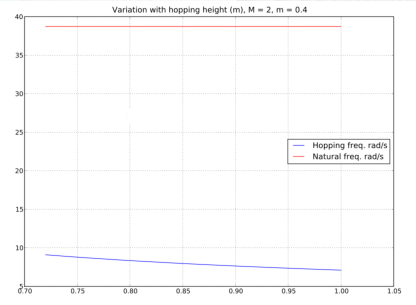
\includegraphics[scale=1.8]{fig/freq_hopheight.pdf}
\caption{Frequency variation with hopping height for M/m = 5}
\label{fig:4_freq_height}
\end{figure}
Fig. \ref{fig:4_freq_height} shows that $\omega_{hop}$ and $\omega_{nat}$ are separated by large gap for the usable range
of values of hopping height. A similar analysis for variation of M also reveals that the two frequencies are separated
by a large gap for all usual values.
\begin{figure}[!h]
\centering
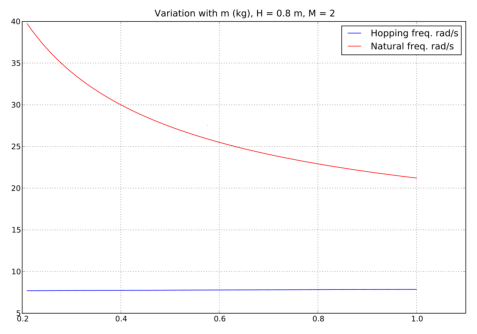
\includegraphics[scale=1.5]{fig/freq_m.pdf}
\caption{Frequency variation with m}
\label{fig:4_freq_m}
\end{figure}
Fig. \ref{fig:4_freq_m} succinctly depicts all the above analysis. As the leg mass increases, the hopping frequency goes
closer to the natural frequency i.e. more impact per unit time. To compound matters, more and more energy is lost per impact
as per Eqn. \ref{eqn:4_eloss}. So the conclusion from impact analysis is that the leg mass should be as low as possible. It is also
seen from Fig. \ref{fig:4_freq_m} that \mbox{m = 0.4 -- 0.6 kg} is a good solution as well as an achievable one. 

\section{Reaction wheel}
\label{sec:4_rewac}
For achieving a running gait with the hopper, it has to be started with the exact initial pitch and horizontal velocity.
For any other initial condition, the hopper is pitch unstable and will not be able to continue the running gait.
As mentioned in \cite{shanmug}, an offset mass acts as a passive stabilization to the pitch attitude of the hopper.
To get rid of this need for exact initial condition which is quite impractical, we design a reaction wheel on the hopper.
This will result in torque coupling on the pitch axis and thus provide an active control over the pitch of the robot.
The coupling equation can be written as,
\begin{equation}
J_{wheel}\;\omega_{wheel} = -(J_{wheel} + J_{body})\;\omega_{body}
\end{equation}
\begin{figure}[!h]
\centering
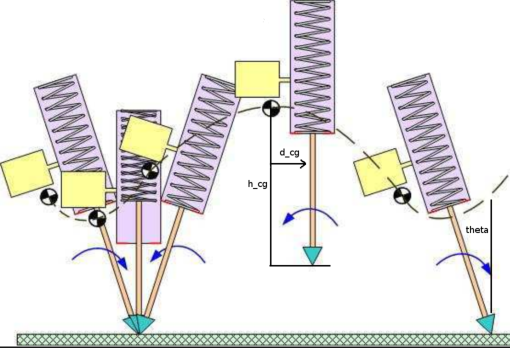
\includegraphics[scale=1]{fig/slom_motion.pdf}
\caption{Stabilizing impact torque due to SLOM}
\label{fig:4_rewac}
\end{figure}
Let us look at the various stages of reaction wheel stabilization,
\begin{itemize}
\item
Let $\theta_{impact}$ be the impact pitch attitude and $\theta_{liftoff}$ be the lift-off attitude. Pitch is measured with respect to
the vertical direction. An upright hopper means a pitch of zero.
\item
From Fig. \ref{fig:4_rewac}, the stabilizing impact torque is given by \mbox{$\tau = m\:v_{impact}\:(h_{cg} sin\:\theta + d_{cg} cos\:\theta)$}. This is a positive torque and generates a pitch up. Also, \mbox{$\omega_{liftoff} = \tau_{impact}\:/J_{body}$}
\item
The angle rotated due to horizontal velocity in the stance phase is $\Delta\:\theta = -v_h\:/h_{cg}\:\Delta\:t$ where $v_h$ is the horizontal velocity. This means
$\theta_{liftoff} = \theta_{impact} + \Delta\:\theta$.
\item
The lift-off pitch needs to be corrected to $\theta_{impact}$ while the hopper is in the air. $\omega_{liftoff}$ might not be enough
to correct this pitch and so we need an additional reaction wheel.
\end{itemize}
The following assumptions were made during the analysis for the reaction wheel,
\begin{itemize}
\item
The reaction wheel is taken as a ring with mass of 1.5 kg concentrated at the rim.
\item 
It is easy to see that for any given horizontal velocity, there exists a particular impact pitch which results in stable gait without a reaction wheel. Our objective is thus to go to this impact pitch angle from any
given initial condition such as a zero pitch angle.
\item
We consider the case where the pitch is such that we have no horizontal velocity and no stabilization impulse from the ground. This pitch is reoriented to 30 degrees within one hop which corresponds to a huge horizontal velocity of 13.5 m/s. The stable pitch will be less than this for lower velocities. In actual operation
there will be large reaction wheel torques only while converting the initial condition into a stable
running gait. After that there will only be small control torques about the stable pitch angle.
\item
We assume a trapezoidal profile for $\omega_{wheel}$ with length of the plateau taken as $T_{air}/2$. The acceleration phase is
$T_{air}/5$ on either side. This means that we finish the reorientation task within 9/10 ths of the time that the hopper remains in the air in the first hop ($T_{air} = t_1 + t_3$ from Section \ref{sec:4_impact}).
\end{itemize}


\begin{figure}[!h]
\centering
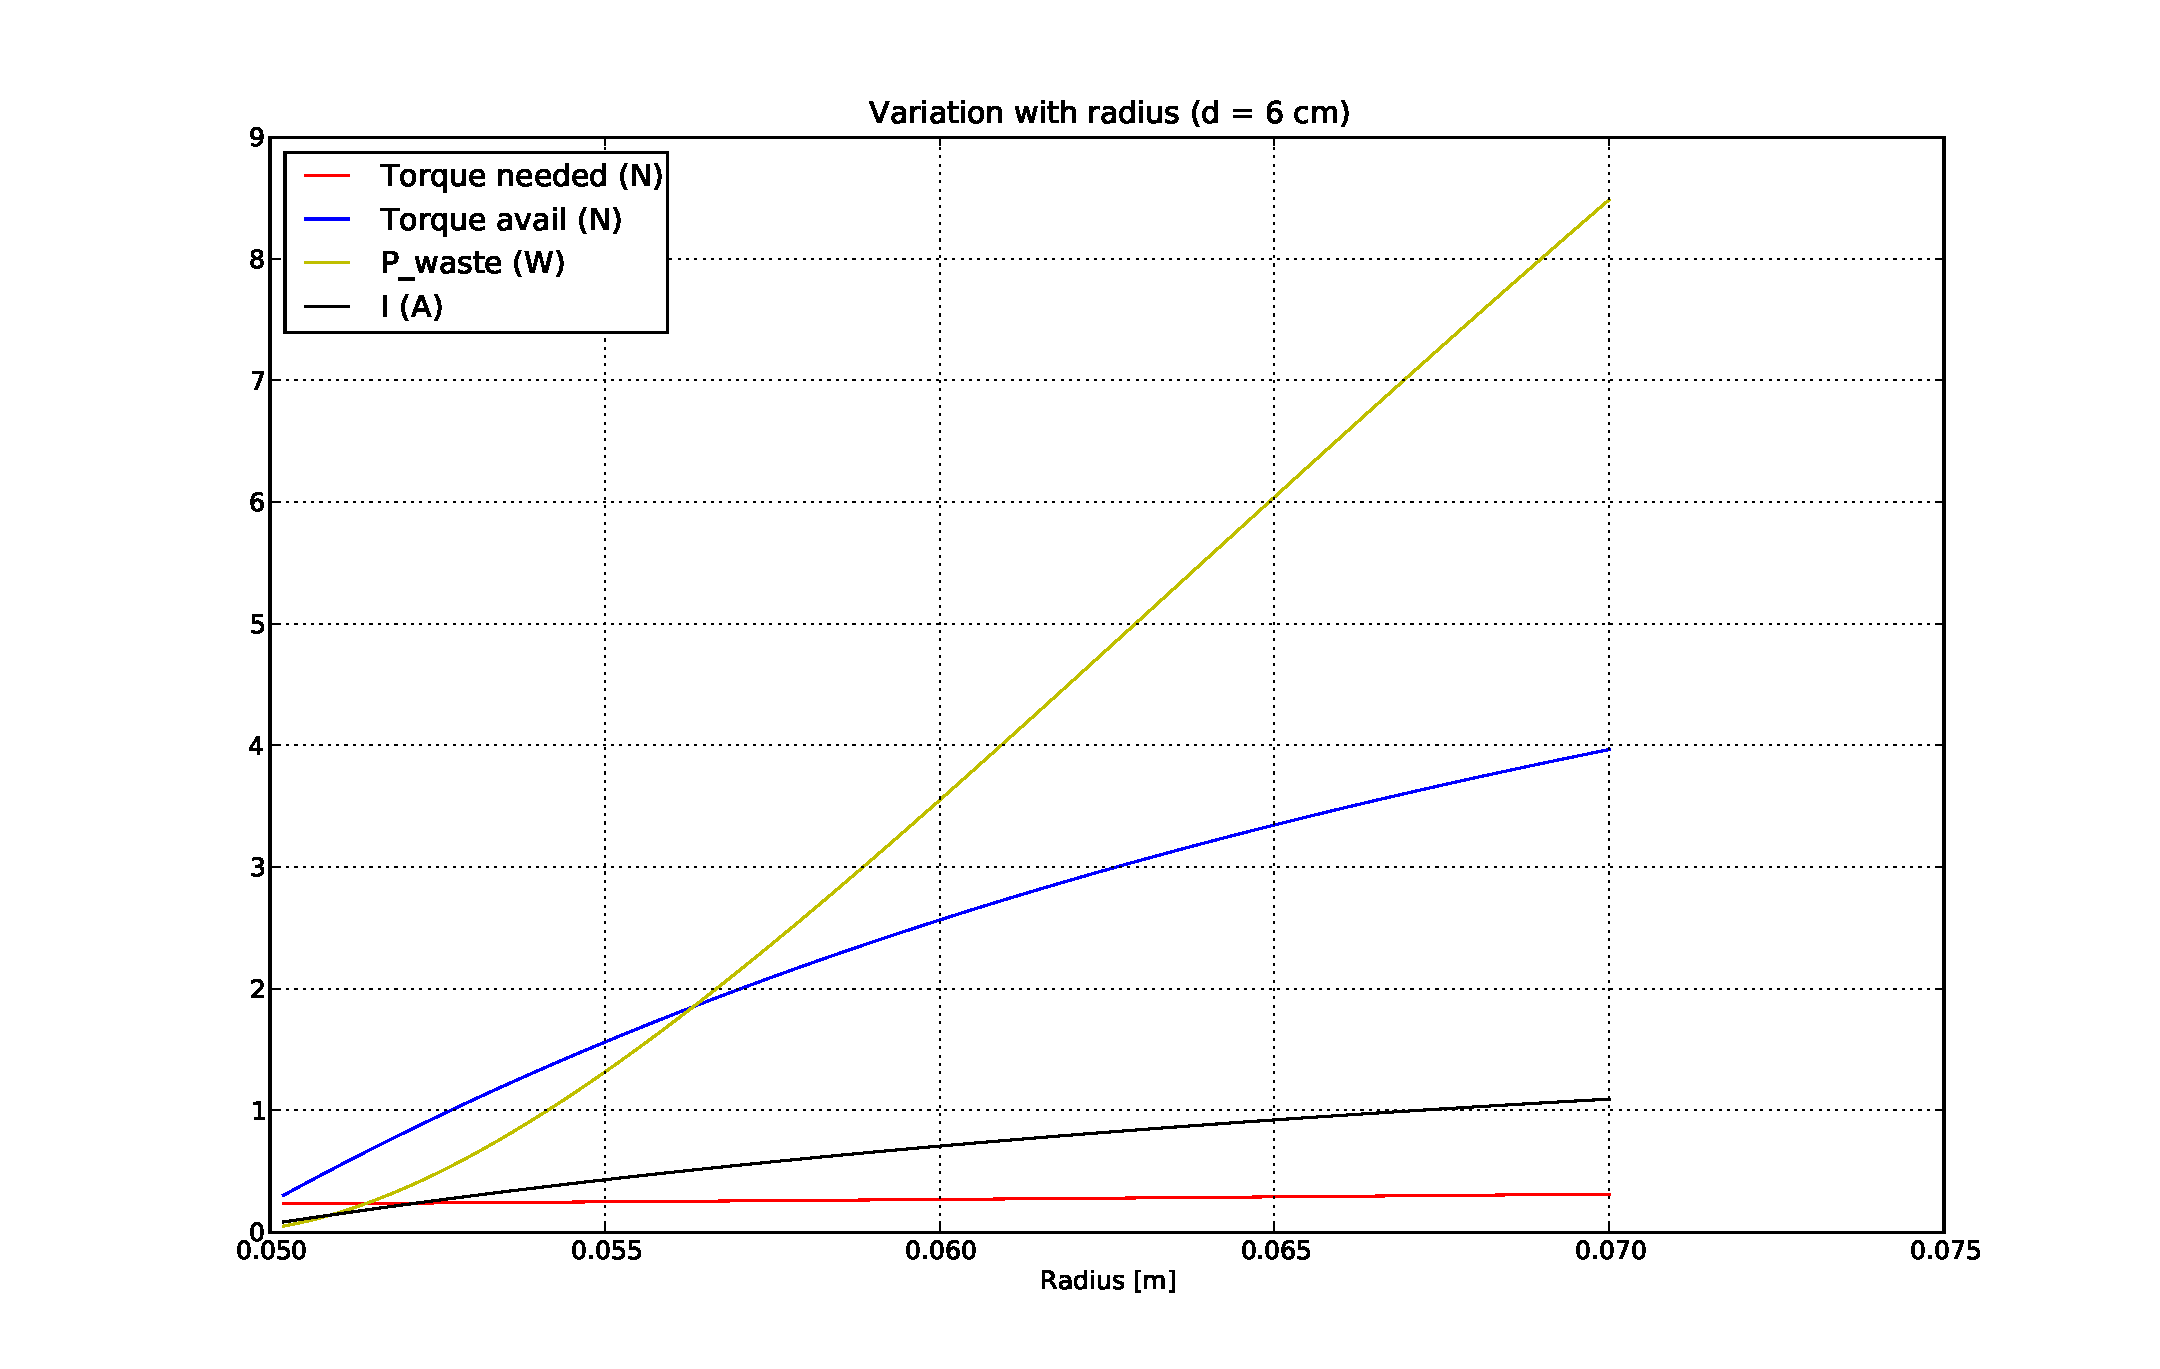
\includegraphics[scale=1.4]{fig/rewac_radius.pdf}
\caption{Torque requirements vs wheel radius}
\label{fig:4_rewac_radius}
\end{figure}
\begin{figure}[!h]
\centering
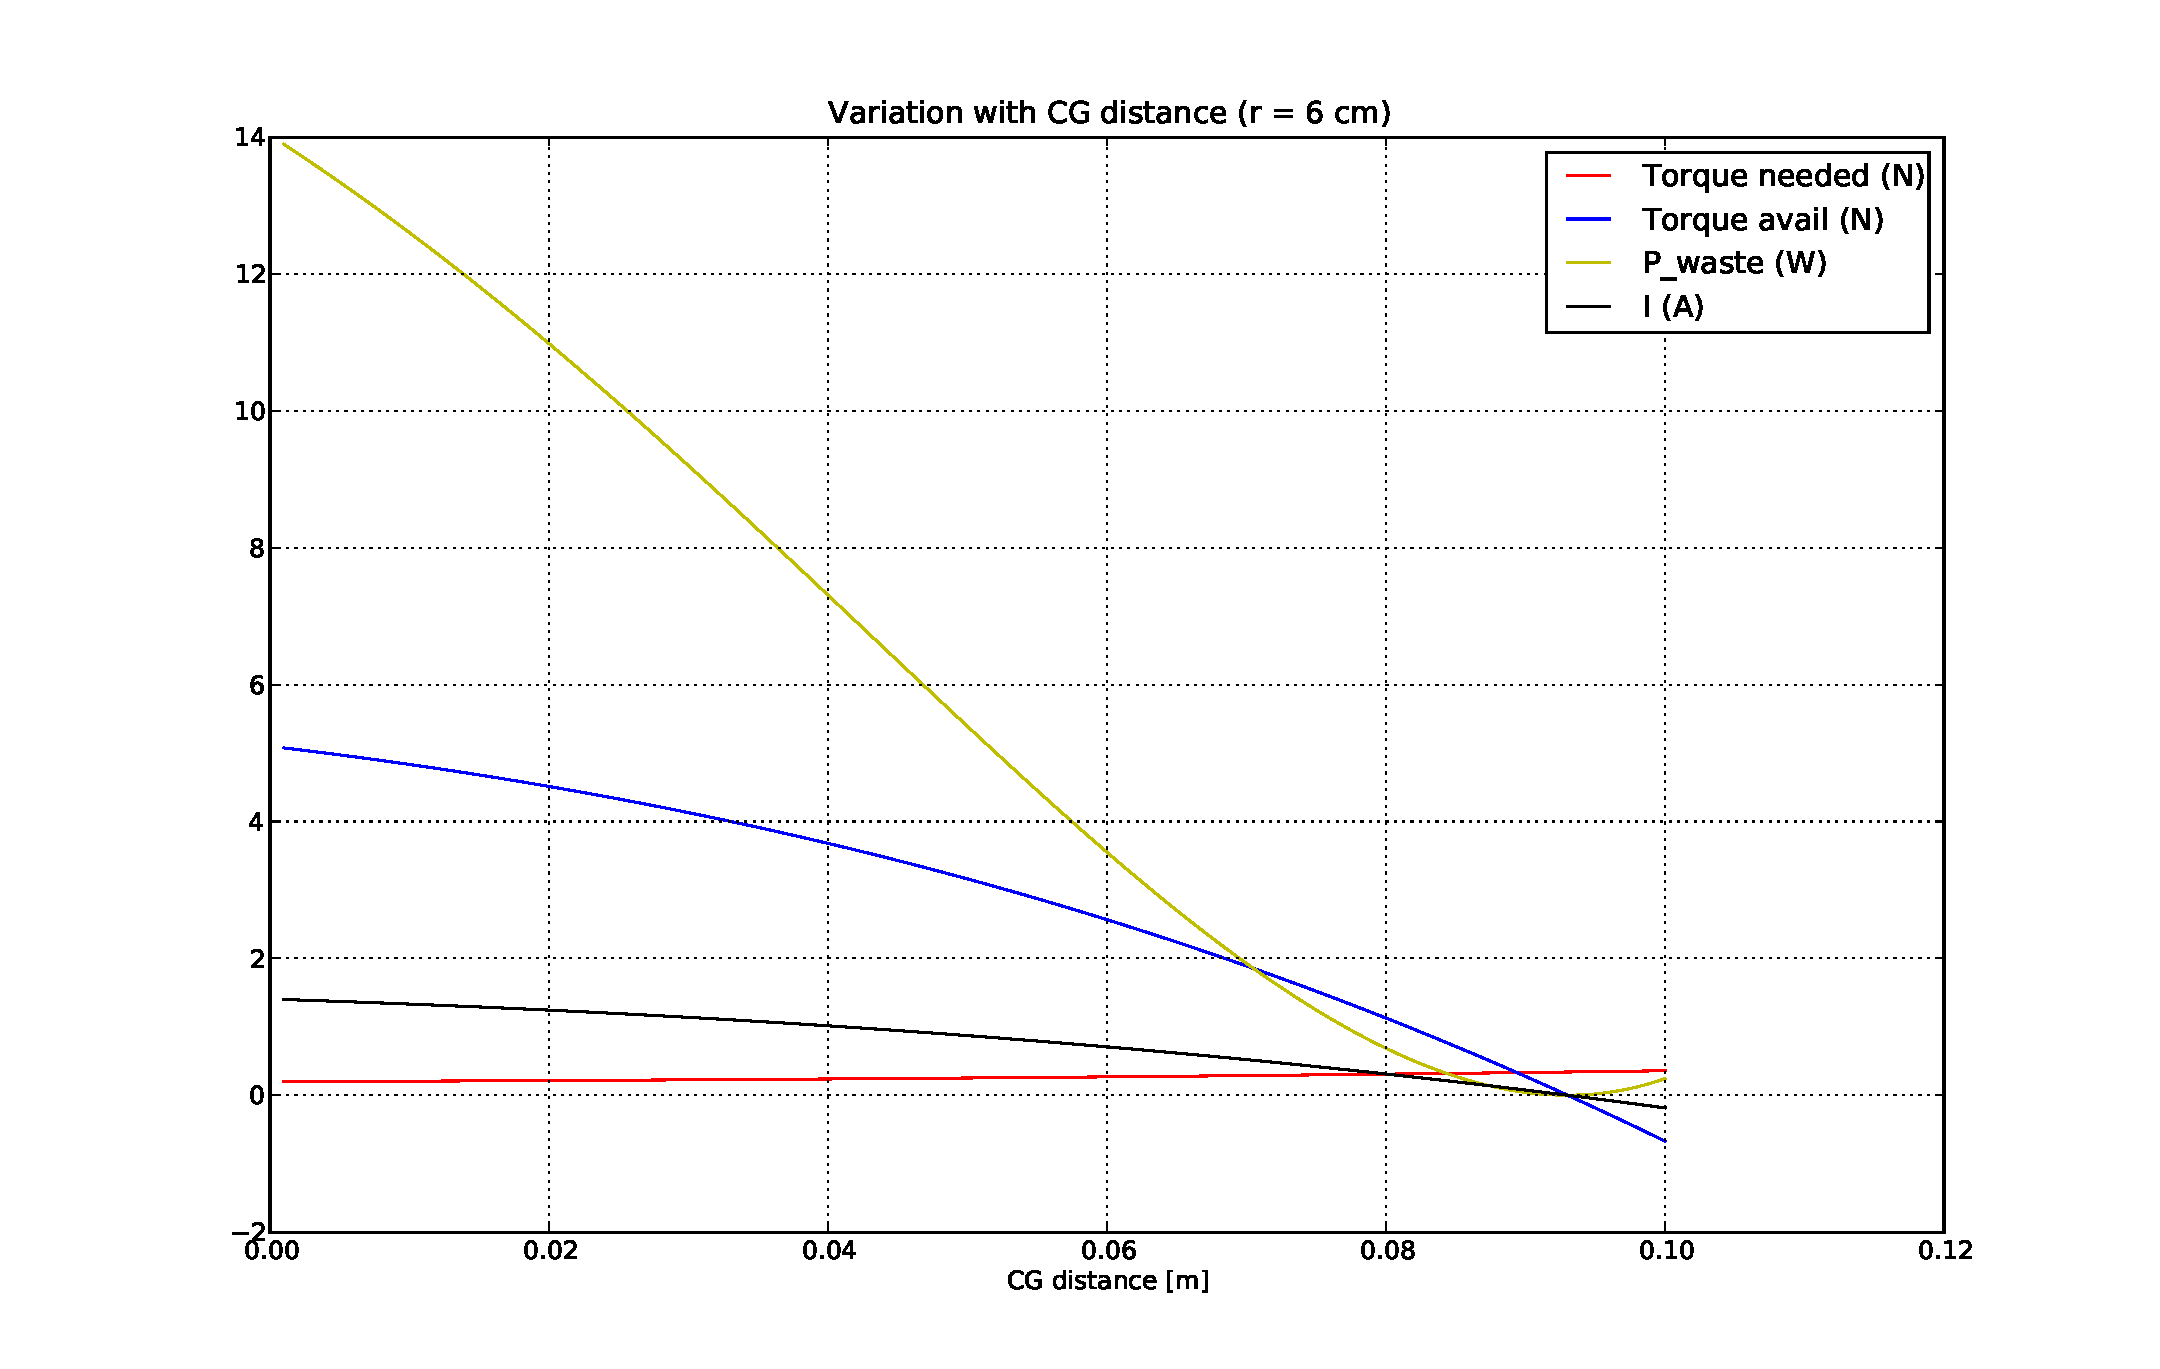
\includegraphics[scale=1.4]{fig/rewac_dist.pdf}
\caption{Torque requirements vs C.G. offset}
\label{fig:4_rewac_dist}
\end{figure}

\subsection*{Results}
Figs. \ref{fig:4_rewac_radius} and \ref{fig:4_rewac_dist} have been plotted for distance of C.G. = 6 cms and
radius of the reaction wheel taken as 6 cm (mass = 1.5 kg). We can see that the required torque for reorientation as mentioned in above is around 500 mNm with output power being around 1.5 W.

\section{Choosing Components}
\subsection*{Reaction wheel motor}
Figs. \ref{fig:4_rewac_dist} and \ref{fig:4_rewac_radius}, were plotted for a 2342CR024 motor. We bump up
the gear ratio to achieve a higher available torque as compared to the necessary torque. There is a trade off
here because we also want a particular value of $\omega$ for reorientation. We thus choose to suffer on the
amount of wasted power to achieve these dual objectives. The gear-box thus chosen is one with a standard 139 : 1 ratio. The motor was chosen by looking at the currents required for different motors. The current required
for this motor is around 1.2 A.

\subsection*{Drive motor}
We look at Fig. \ref{fig:4_torque2mass} to choose the drive motor. For the purposes of design, we take common values of worm-worm wheel diamter ratio (0.5), pressure angle (20 deg), helix angle for worm (25 deg) and co-efficient
of friction $\mu = 0.3$. The torque required from the motor is not more than 200 mNm. The total power required
for this task is about 4.5 W. We choose the same 2342CR024 motor for this task. The gear box is taken as a
43 : 1
standard one to ensure that we are operating at the rated motor speed. This results in less energy wastage. There need not be any optical encoders for this motor as we will be measuring the velocity of the extension using encoders at the band drive. The currents for this operation are always below 1.5 A. Hence we can use a relatively small motor driver like Texas Instruments DRV 8801 to drive this motor.


